
\section{\rqthree}
\label{rq3:method}


\todo{The last method is too short}


\newcommand{\mewe}{MEWE\xspace}

% What do we do
To answer RQ3, we use the variants generated for the programs of \corpussodium and \corpusqrcode corpora, we take $2 + 5$ programs interconnecting the LLVM bitcode modules (mentioned in \autoref{table:corpora}). We illustrate the protocol to answer RQ3 in \autoref{diagrams:protocol:rq3} starting from the creation of the programs' population.

\begin{figure}[h]
    \centering
    \includegraphics[width=0.8\linewidth]{diagrams/Rq3.pdf}
    \caption{Multivariant binary creation and workflow for RQ3 answering.}
    \label{diagrams:protocol:rq3}
\end{figure}

% Why do we do it ?
In RQ3, we study whether the created variants can be used in real-world applications and what properties offer the composition of the variants as \termidx[multivariant ]{Software!Multivariant}binaries. We build \termidx[multivariant ]{Software!Multivariant}binaries (according to \autoref{def:EP}), and we deploy and execute them at the Edge. 
The usage of Edge-Cloud computing platforms to answer RQ3 is motivated by two reasons. First, it is an emerging technology. 
Using Wasm as an intermediate layer is better in terms of startup and memory usage, than containerization or virtualization \cite{pMendkiServerless, 1244493Jacobsson}. 
This has encouraged edge computing platforms like Cloudflare or Fastly to adopt \wasm to deploy client applications in a modular and sandboxed manner  \cite{CloudflareWasm, FastlyWasm}.
Second, Edge-Cloud computing platforms are shown to be not completely secure \cite{Narayan2021Swivel} and multivariant execution offers a preemptive technique against predictable behaviors such as execution time.




%The workflow starts by using the programs' population of each program generated in RQ1 to create the \termidx[multivariant ]{Software!Multivariant}binaries. We deploy the \termidx[multivariant ]{Software!Multivariant}binaries at the Edge, and we collect their execution times. We measure the differences for the execution times on the edge. Then, we discuss how \termidx[multivariant ]{Software!Multivariant}binaries contribute to less predictable timing side-channels.

\subsection*{Metrics}

To answer RQ3, we build \termidx[multivariant ]{Software!Multivariant}\wasm binaries (see \autoref{def:EP}) meant to provide execution path randomization.
We use the execution time of the \termidx[multivariant ]{Software!Multivariant}binaries to answer RQ3. We use the same metric defined in \autoref{metric:time} for the execution time of \termidx[multivariant ]{Software!Multivariant}binaries.

\subsection*{Protocol}


%\todo{too fast. tell the reader why you need HTTP now}
We answer RQ3 by analyzing a real-world scenario. We run our experiments for RQ3 on the Edge. 
Edge applications are designed to be deployed as isolated HTTP services, having one single responsibility that is executed at every HTTP request. This development model is known as serverless computing, or function-as-a-service \cite{shillaker2020faasm,Narayan2021Swivel}. 
We deploy and execute the \termidx[multivariant ]{Software!Multivariant}binaries as end-to-end HTTP services on the Edge and we collect their execution times.
To remove the natural jitter in the network, the execution times are measured at the backend space, \ie we collect the execution times inside the Edge node and not from the client computer. 
Therefore, we instrument the binaries to return the execution time as an HTTP header. 

We do the collection of the execution times twice, for the original program and its \termidx[multivariant ]{Software!Multivariant}binary. We deploy and execute the original and the \termidx[multivariant ]{Software!Multivariant}binaries on 64 edge nodes located around the world. In \autoref{diagrams:protocol:rq3:map} we illustrate the word wide location of the edges nodes.


\begin{figure}[h]
    \centering
    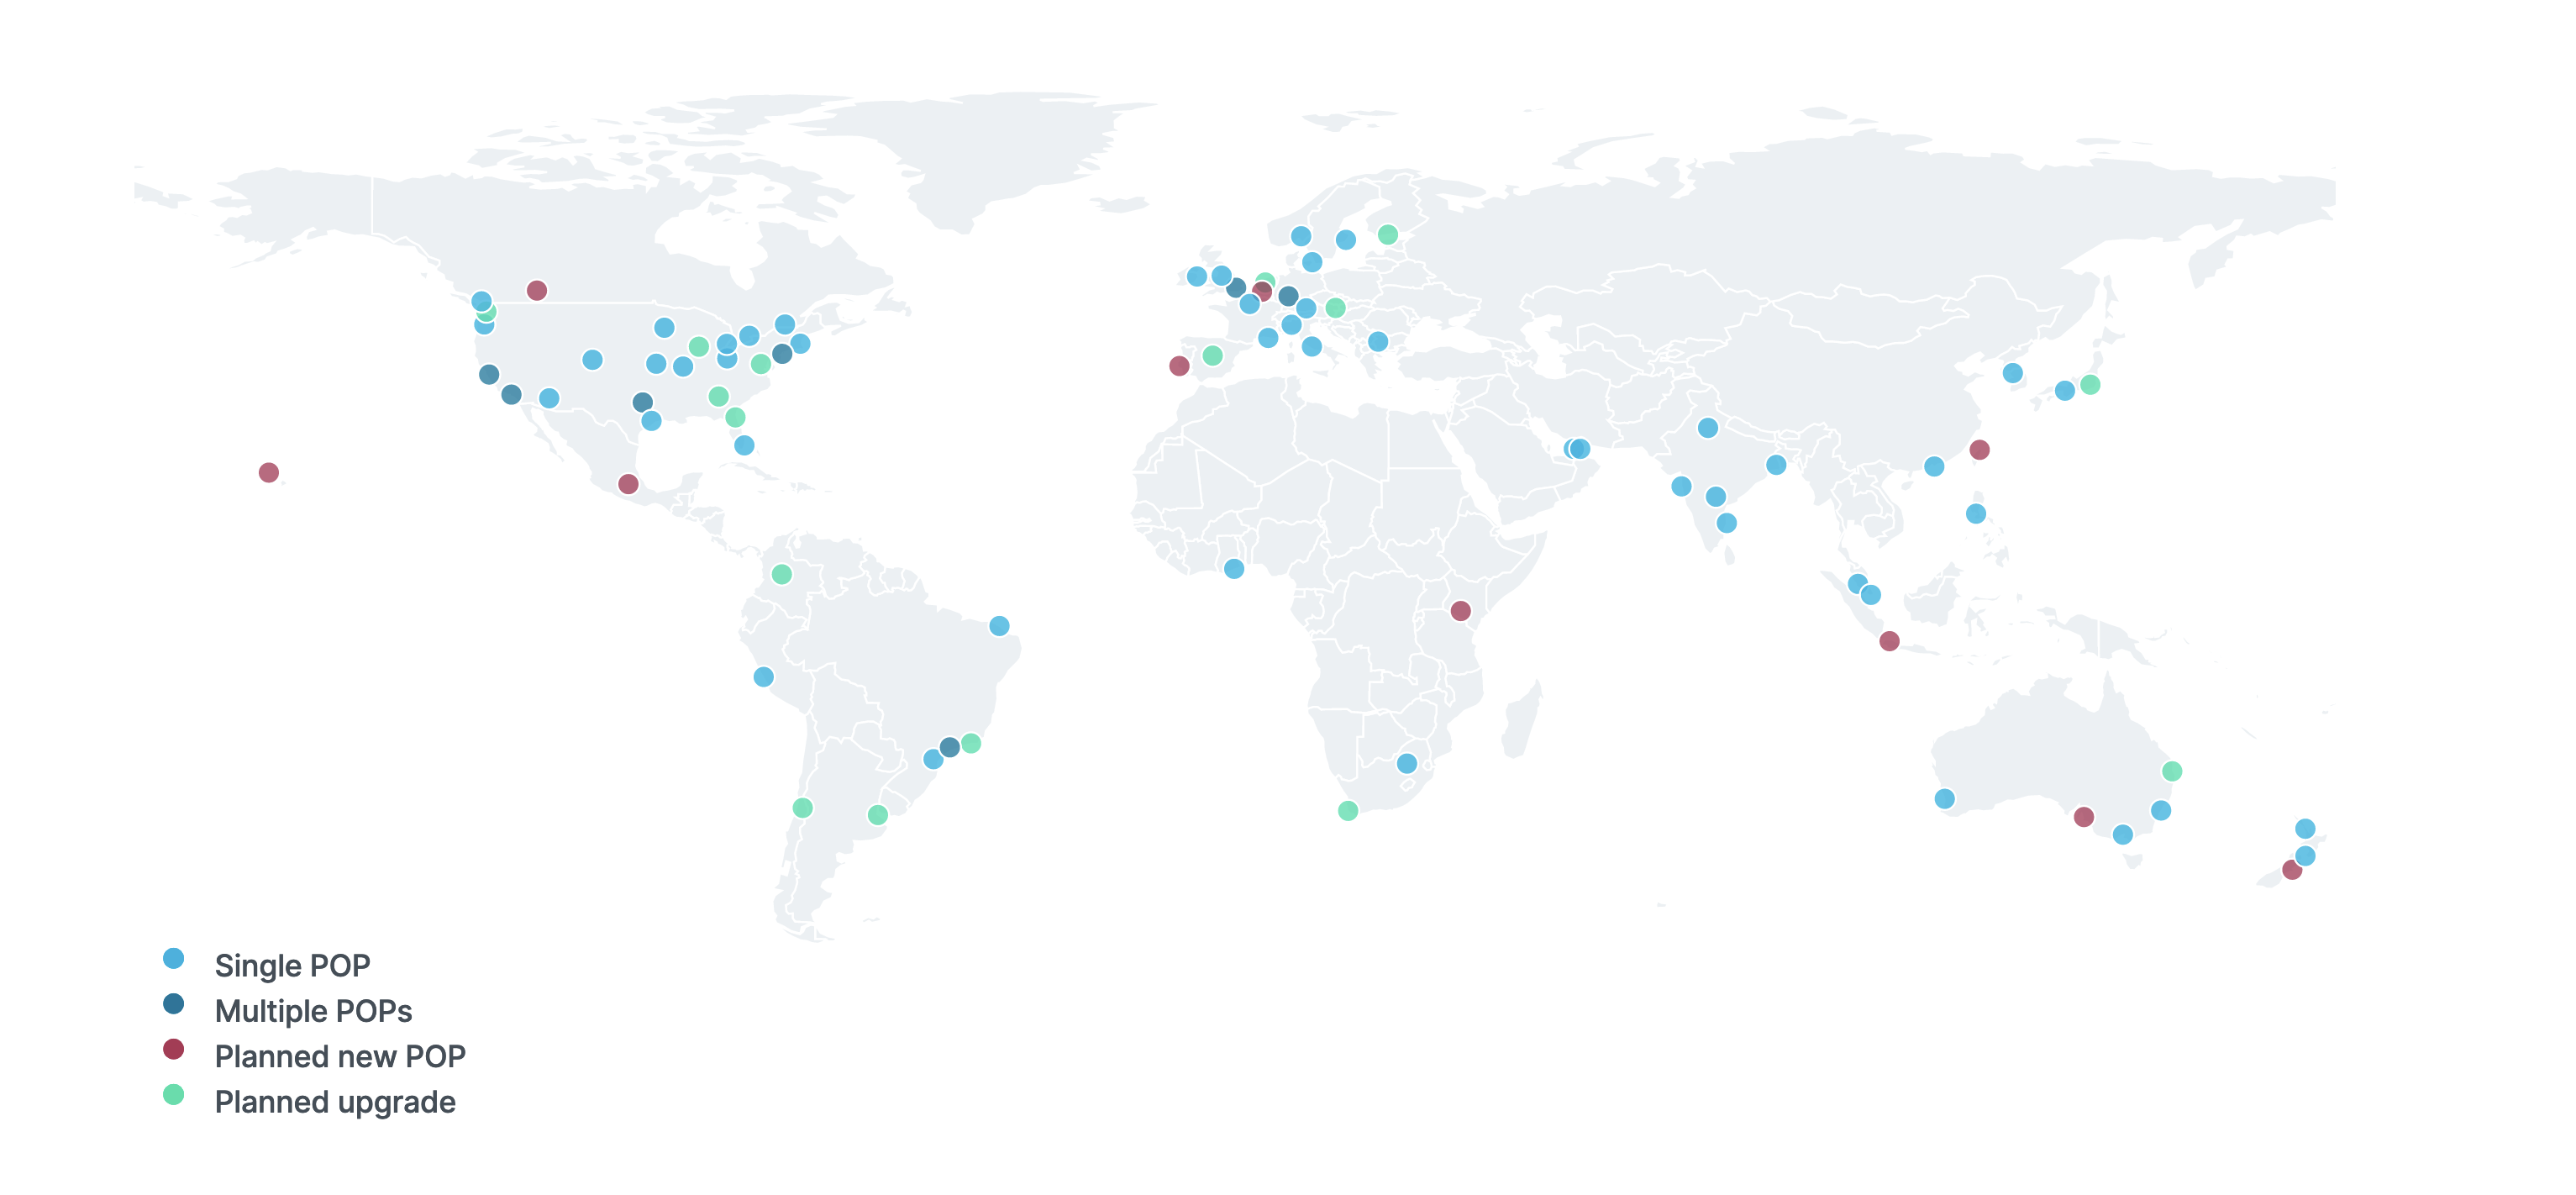
\includegraphics[width=\linewidth]{diagrams/pops.png}
    \caption{Screenshot taken from the Fastly Inc. platform used in our experiments for RQ3. Blue and darker blue dots represent the edge nodes used in our experiments.}
    \label{diagrams:protocol:rq3:map}
\end{figure}



We collect 100k execution times for each binary, both the original and \termidx[multivariant ]{Software!Multivariant}binaries. The number of execution time samples is motivated by the seminal work of Morgan \etal \cite{morgan2015web}. 
We perform a Mann-Withney U test \cite{mann1947} to compare both execution time distributions. 
If the P-value is lower than 0.05, the two compared distributions are different.